\DeclarePairedDelimiter\ceil{\lceil}{\rceil}
\DeclarePairedDelimiter\floor{\lfloor}{\rfloor}

%CHAPTER
\chapter{Implementace modulu}
Během analýzy celého programu bylo potřeba vybrat nejvhodnější knihovnu pro generování souborů PDF a tu následně integrovat s~předem vybraným parserem. Pro snadnější integraci byly vytvořeny nové třídy.
\section{Adresářová struktura modulu}
Adresářová struktura modulu na serveru vypadá následovně:
\begin{itemize}
	\item \verb|config| -- Adresář obsahující konfigurační soubor configuration.xml, ve kterém jsou uložena často měněná data (rok konference aj.).  
	\item \verb|img| -- Adresář obsahující obrázky použité v~dokumentu (logo konference TSD).
	\item \verb|lib| -- Adresář obsahující zdrojové kódy knihoven třetích stran (generátor a parser).
	\item \verb|src| -- Adresář obsahující zdrojové kódy vytvořené autorem bakalářské práce.
	\item \verb|orlib.php| -- Hlavní soubor modulu obsahující všechny tři stěžejní funkce modulu.
\end{itemize}
%SECTION
\section{Implementované třídy}
Pro modul jsem vytvořil sedm tříd, které integrují pomocné knihovny pro generování a zpracování souborů PDF (vytváření formulářových prvků, konstanty aj.).
%SUBSECTION
\subsection{Výčtové typy}
\textbf{Výčtový typ} (neboli \textbf{Enum}) je datový typ určený pro uložení konstant programu, kdy každé z~těchto konstant je přiřazena jedna instance výčtu. Ve vytvářeném modulu byly použity čtyři výčtové typy. 
\par
Výčtový typ \textbf{Instruction} uchovává konstanty využité při generování titulku a informací během vyplňování formuláře. Tyto konstanty reprezentují celkem čtyři části dokumentu (záhlaví, titulek dokumentu, jméno recenzenta a instrukční text pro vyplňování formuláře).
\par
Výčtový typ \textbf{FormElements} slouží pouze pro rozlišení použitých objektů na základní prvky formuláře. Zde byly použity výběrové tlačítko a textové pole.
\par
Ve výčtovém typu \textbf{TextareaInfo} jsou uloženy veškeré hodnotící parametry, které jsou reprezentovány jako textová pole, a pomocné funkce. Každý hodnotící parametr je zde určen třemi konstantami (jednoznačný identifikátor, název a jeho popis). Dále se tu vyskytují dvě konstanty využité při vytváření formulářového prvku pomocí HTML kódu. Tyto konstanty jsou využity i při následném zpracování dokumentu pro všechny formulářové prvky reprezentované jako textová pole. Byla zde vytvořena i funkce \textit{getNotNeededConstants} pro získání nepovinných hodnotících parametrů.
\par
Výčtový typ \textbf{RadiobuttonInfo} je téměř totožná s~třídou \textbf{TextareaInfo} s~tím rozdílem, že hodnotící parametry jsou reprezentovány jako skupina výběrových tlačítek.
%SUBSECTION
\subsection{Elements}
Hlavním důvodem vzniku této třídy byla snaha nevytvářet formulářové prvky přímo v~hlavní funkci \textit{generate\_offline\_review\_form}, ale použít nově vytvořené metody. Pomocí implementovaných metod lze vytvářet textová pole, výběrová tlačítka, textové části dokumentu a načítat vědecký příspěvek.
%SUBSECTION
\subsection{TextConverter}
V~některých případech jsou název vědeckého příspěvku nebo jméno recenzenta příliš dlouhé, a proto narušuje vzhled výsledného dokumentu. Problém může nastat i při chybě programátora, pokud by byl instrukční text příliš rozsáhlý. Proto byla vytvořena třída \textbf{TextConverter}, která má za úkol nejdříve zkontrolovat předaný text a porovnat ho se stanovenými konstantami určujícími maximální délku textu. Pokud je rozsah textu delší než stanovená délka, vypočte se následně potřebný font pro vykreslení celého textu pomocí vzorce \eqref{eq:font_size}. Délka se porovnává se stanovenými konstantami určujícími minimální velikost fontu. 
\begin{equation}
%newFontSize = \floor*{\frac{maxTextLength}{textLength} \cdot fontSize} \label{eq:font_size}
h\textsubscript{n} = \floor*{\frac{l\textsubscript{max}}{l} \cdot h}, \\
\label{eq:font_size} 
\end{equation}
kde \textit{h\textsubscript{n}} je nově vypočtená velikost fontu, \textit{l\textsubscript{max}} je maximální délka kontrolovaného textu, \textit{l} je aktuální délka kontrolovaného textu a \textit{h} je aktuální velikost fontu.

Pokud je vypočtený font je menší než předem stanovený minimální font, je text zkrácen na velikost vypočtenou pomocí vzorce  \eqref{eq:text_length} a doplněn třemi tečkami na jeho konci. 

\begin{equation}
%newLength = \floor*{\frac{oldFontSize}{minFontSize} \cdot textLength} \label{eq:text_length}
l\textsubscript{n} = \floor*{\frac{h\textsubscript{p}}{h\textsubscript{min}} \cdot l}, \\
\label{eq:text_length}
\end{equation}
kde \textit{l\textsubscript{n}} je nově vypočtená délka kontrolovaného textu, \textit{h\textsubscript{p}} je původní velikost fontu, \textit{h\textsubscript{min}} je minimální velikost fontu a \textit{l} je délka kontrolovaného textu.
%SUBSECTION
\subsection{ConfigurationData}
Třída načítá veškerý obsah konfiguračního souboru, který následně ukládá do svých proměnných. Data uložená v~konfiguračním souboru slouží pro nastavení textu vodoznaku a jako informační text pro uživatele.
%SECTION
\section{Generátor}
Generátor by měl být při vytváření dokumentu PDF rychlý, vykreslit co nejpřesněji prvky webového formuláře do vygenerovaného dokumentu a nebýt implementačně náročný.
%SUBSECTION
\subsection{TCPDF versus mPDF}
Při analyzování dostupných PHP knihoven pro generování souborů PDF byly nalezeny dvě vyhovující knihovny, které splňují potřebnou funkcionalitu. Po vytvoření jednoduchého souboru obsahujícího základní formulářové prvky jsem se rozhodl, že použiji knihovnu \textbf{mPDF} pro generování souborů PDF. Důvody této volby jsou popsány níže.
\par
Za jeden z~důležitých faktorů lze označit podporu \textit{CSS3} (Cascading Style Sheets 3) u~\textbf{mPDF}, díky čemuž lze dosáhnout perfektního nastavení stylů pro jednotlivé objekty v~dokumentu. Naproti tomu \textbf{TCPDF} nepodporuje značné množství CSS parametrů, například parametr určující šířku vnějšího okraje prvku, a pro dosažení obdobného výsledku je zapotřebí značné množství jiných parametrů definujících styl prvku.
\par
Důležitým faktorem při vytváření dokumentu PDF je rychlost generování a paměťová náročnost. V~tabulce \ref{tab:table_generators} lze vidět porovnání knihoven pro dva  soubory PDF, kdy první PDF obsahovalo hlavně kaskádové styly, zatímco v~druhém PDF byla vytvořena tabulka s~více jak tisíci záznamy.
\begin{table}[h!]
\centering
\begin{tabular}{|l|l|l|l|l|} 
\hline
\textbf{Název} & \multicolumn{2}{l|}{\textbf{Komplexní PDF}} & \multicolumn{2}{l|}{\textbf{Dlouhé PDF}}  \\ 
\hline
               & \textbf{Paměť [MB]} & \textbf{Čas [ms]}     & \textbf{Paměť [MB]} & \textbf{Čas [ms]}   \\ 
\hline
TCPDF (v6.2.13)          & 74                  & 35944                 & 2,3                 & 96350               \\ 
\hline
mPDF   (v7.1.6)           & 14                  & 11316                 & 22,5                & 4120                \\
\hline
\end{tabular}
\caption{Tabulka časové náročnosti a využité paměti při generování}
\label{tab:table_generators}
\end{table}
\par
Posledním a zároveň rozhodujícím faktorem je psaní PHP kódu pro vykreslování obsahu, kdy při vytváření kódu u~\textbf{mPDF} se využívá minimum funkcí pro nastavení parametrů souboru PDF jako jsou například metadata, zatímco veškeré zobrazené elementy a text jsou psány v~jazyce HTML, se kterým se snadno pracuje. V~mPDF lze snadno měnit parametry jednotlivých elementů, což bude oceněno hlavně u~parseru. U~\textbf{TCPDF} se zobrazovaný obsah vkládá pomocí předem vytvořených funkcí, přičemž tyto funkce mohou obsahovat mnoho parametrů, které si uživatel obtížně zapamatuje a vždy bude potřebovat patřičnou dokumentaci pro správné použití, což bude zabírat mnoho času při vyvíjení nových modulů.
\par
Na závěr porovnání lze říci, že ve většině případů je vhodné využít pro generování souborů PDF knihovnu \textbf{mPDF}. Pokud by bylo nutné vytvořit dokument například ve stylu knihy s~nulovým využitím CSS stylů a potřebou kvalitního vysázení textu, pak je lepší použít knihovnu \textbf{TCPDF}. 

%SUBSECTION
\subsection{Popis vytvoření dokumentu}
Na samotném začátku generování jsou vytvořeny instance tříd. U~instance třídy \textbf{ConfigurationData}, proběhne i načtení dat z~konfiguračního souboru XML. Dále jsou vytvořeny proměnné reprezentující název vybraného dokumentu a informace o~nahrání vyplněného dokumentu do webového portálu konference TSD. Před samotným začátkem generování je do modulu importováno CSS nastavení pro vzhled celého dokumentu.
\par
V~první části generování probíhá vytvoření záhlaví. V~celém dokumentu je použit font \textit{Helvetica}, pouze výjimečně je zařazen font \textit{Times New Roman}, například pro titulek dokumentu a text se stylem \textit{Bold}. Do záhlaví je vložen identifikátor recenze doplněn o~název hodnoceného vědeckého příspěvku, který je případně zkrácen na určitou délku, pokud nesplňuje limity nastavené ve třídě \textbf{TextConverter}, a logo konference TSD. 
\par
V~druhé části generování probíhá vložení vodoznaku do celého dokumentu, uložení jednoznačného identifikátoru jak vědeckého příspěvku v~recenzním řízení, tak i hodnotícího příspěvku do příslušných metadat dokumentu. Na první stránce dokumentu je vykreslen titulek s~identifikátorem hodnoceného vědeckého příspěvku, název hodnoceného vědeckého příspěvku (případně zkrácen stejně jako u~záhlaví), jméno recenzenta a doprovodný text při vyplňování hodnotícího formuláře. Pod tímto textem je vykreslena první část hodnotícího formuláře, která obsahuje osm skupin výběrových tlačítek a jedno textové pole.
\par
V~poslední části probíhá vykreslování zbylých čtyř textových polí, kde dvě poslední z~nich jsou nepovinná. Za hodnotícím formulářem je vložen kompletně celý hodnocený vědecký příspěvek.
%SUBSECTION
\subsection{Nedostatky v~mPDF}
\label{subsec:nedostatky_v_mpdf}
Při vytváření dokumentu byly nalezeny dvě chyby znemožňující úplné vykreslení celého dokumentu. Níže jsou tyto chyby popsány i s~návrhem jejich řešení.
\par
První nedostatek byl zjištěn na úplném začátku implementace generátoru, kdy při vkládání textových polí do formuláře se po přeložení kódu nevytvořil žádný dokument. Při zkoumání zdrojového kódu knihovny a vytvoření testovacích dokumentů bylo zjištěno, že knihovna neumožňuje použít textové pole, pokud se při jeho vytvoření nezadá vkládaný text. Proto bylo nutné upravit kód knihovny, konkrétně ve vykreslování textového pole. Aby bylo možné takto upravovat zdrojový kód knihovny, nesmí být knihovna pod licencí a naopak musí  být alespoň pod licencí dovolující úpravy, například \textit{GNU General Public License} verze 2, pod kterou je licencována i mPDF. Pro vyřešení tohoto problému byl přidán mechanismus, který při vytváření prázdného textového pole přidá znak \uv{\textbf{a}} (viz \ref{lst:elements_a}) a posléze je v~knihovně při vykreslování textového pole tento znak odstraněn, což nemá vliv na jakýkoliv jiný znak či slova než zmiňovaný znak \uv{\textbf{a}}, viz obrázek \ref{lst:mpdf_a}.
\begin{lstlisting}[caption = {Dočasné přiřazení znaku \uv{\textbf{a}} do textového pole (Elements.php)}, label = {lst:elements_a}, captionpos=b]
if($textarea_text == '') $textarea_text = 'a';
\end{lstlisting}
\begin{lstlisting}[caption = {Odstranění znaku \uv{\textbf{a}} z~textového pole (Mpdf.php)}, label = {lst:mpdf_a}, captionpos=b]
if (isset($objattr['text']) && $objattr['text'] != 'a') {
	$texto = $objattr['text'];
}
else $texto = '';
\end{lstlisting}
\par
Druhý nedostatek byl nalezen při testování zkracování délky textu titulku, pokud překročí nastavenou mez. V~aktuální verzi PHP se vyskytuje problém, který zneplatňuje některé znaky v~kódování UTF-8. Pokud je například vytvořen nový uživatel se jménem obsahující například znak \uv{\textbf{ř}}, pak se tento znak nepřevede správně a bude vykreslen jako neznámý znak. Bohužel generování dokumentu neprobíhalo správně, protože knihovna mPDF tyto znaky nerozpoznala, a proto výsledek vždy skončil chybou. Ze všech vyzkoušených možností, jako například změna kódování textu titulku nebo nahrazení neplatných znaků prázdnými, fungovala pouze jedna, a to nastavení atributu ignore\_invalid\_utf8 na \textit{true} u~proměnné třídy \textit{Mpdf} (viz obrázek \ref{lst:ignore_invalid_utf8}).
\begin{lstlisting}[caption = {Nastavení atributu ignore\_invalid\_utf8 (orlib.php)}, label = {lst:ignore_invalid_utf8}, captionpos=b]
$mpdf->ignore_invalid_utf8 = true;
\end{lstlisting}
\par
Nejzávažnější nedostatek knihovny mPDF byl objeven na samém konci testování. Bylo testováno především slučování hodnotícího formuláře s~vědeckými příspěvky. Vědecké příspěvky byly uloženy ve formátu PDF v~různých verzích, nejčastěji verze 1.4 až 1.6. Testování probíhalo perfektně pro PDF verze 1.4, bohužel pro novější verze už slučování neprobíhalo správně a modul generoval výjimku. Důkladným zkoumáním mPDF knihovny bylo zjištěno, že pro slučování souborů PDF se využívá podpůrná knihovna \textbf{FPDI}, která funguje pouze pro soubory PDF do verze 1.4. V~kapitole \ref{subsec:nova_PDF_merge_knihovna} je popsán postup řešení tohoto nedostatku, který zapříčiňuje nefuknční generování hodnotícího dokumentu PDF.

%SUBSECTION
\subsection{Nová knihovna pro slučování souborů PDF}
\label{subsec:nova_PDF_merge_knihovna}
Jedna z~podmínek pro generující knihovnu je umět vkládat hodnocený vědecký příspěvek do výsledného hodnotícího dokumentu PDF. Protože již implementovaná knihovna FPDI tuto funkci neumožňuje, bude potřeba najít jinou knihovnu splňující slučování dokumentů PDF. Nově zvolená knihovna by měla být kompatibilní s~knihovnou mPDF.
\par
Po rozsáhlém průzkumu byla nalezena pouze jedna PHP knihovna, která dokáže slučovat dokumenty PDF verze 1.4. Je jí knihovna \textbf{TCPDI parser}, která je součástí knihovny \textbf{TCPDI}, která dokáže slučovat PDF do verze 1.7.
\par
Následně byla knihovna FPDI nahrazena TCPDI parserem a otestována na několika testovacích souborech PDF s~rozdílnou verzí PDF. Výsledek sloučení nebyl dostatečně kvalitní. Všechny použité styly nebyly přeneseny do výsledného PDF, odsazení textu bylo natolik špatné, že občas byl text posunutý mimo stránku.  Bohužel veškeré přílohy, jako jsou například obrázky, komentáře nebo vzorce, nebyly přítomny ve výsledném dokumentu PDF. Na základě těchto problémů bylo rozhodnuto změnit generovací knihovnu. 

%SUBSECTION
\subsection{Změna knihovny pro generování souborů PDF}
Změna knihovny pro generování souborů PDF byla nutná z~důvodu nedokonalosti mPDF při slučování více souborů PDF. Při testování byla objevena nová knihovna TCPDI, která rozšiřuje již existující knihovnu TCPDF o~nové funkce při slučování dvou či více souborů PDF. 
\par
Pro zprovoznění TCPDI je nutné, aby byla na serveru přítomna knihovna TCPDF, do které bude následně vložen zdrojový kód TCPDI. Zdrojový kód TCPDI se skládá ze tří souborů. První soubor tcpdi\_parser.php obsahuje třídu tcpdi\_parser, která načte data ze souboru PDF a uloží je do předem stanovených struktur. Druhý soubor tcpdi.php obsahuje třídu TCPDI, která rozšiřuje stávající třídu TCPDF a umožňuje slučovat data souborů PDF, ze kterého následně zobrazí výsledný soubor PDF. Třetí a zároveň poslední souborfpdf\_tpl.php obsahuje třídu fpdf\_tpl, která vytváří základy pro znovupoužití PDF objektů v~souboru PDF.
\par
Pro generování obsahu souboru PDF se nevytváří HTML kód, ale využívají se předem vytvořené metody. Jako příklad lze uvést metodu \textit{TextField} třídy TCPDI pomocí které se do souboru vloží textové pole. TCPDI obsahuje metodu, která umožnuje generovat soubor PDF i pomocí HTML kódu, ale z~důvodu nedostatečné podpory kaskádových stylů je tento způsob generování nedoporučován. Proto bylo nutné kompletně přepsat již vytvořený zdrojový kód generátoru a co nejvíce se přiblížit vzhledu souboru PDF jako tomu bylo u~mPDF. Starý zdrojový kód využívající knihovnu mPDF byl zachován pro případ, že bude vytvořena nová knihovna, která bude schopna slučovat soubory PDF nehledě na verzi PDF a bude kompatibilní s~mPDF. 

%SECTION
\section{Parser}
Z~analýzy knihoven pro zpracování dokumentů PDF splnil nutné požadavky pouze \textbf{PDF Parser}. Při implementování parseru bylo zjištěno, že jednotlivé prohlížeče PDF při uložení dokumentu PDF využívají jiné komprimační metody, pracující s~novějšími verzemi PDF pro určité funkce a některé prohlížeče ukládají objekty v~dokumentu na více místech (duplikace, jednou komprimovaně, jednou nekomprimovaně).

%SUBSECTION
\subsection{Popis zpracování dokumentu}
Zpracování dokumentu začíná ihned po jeho nahrání do webového portálu konferenčního systému, kdy se veškerá data předají do PDF Parseru. Před samotnou extrakcí dat jsou pomocí TCPDF parseru, který je součástí PDF Parseru, data rozdělena na objekty pomocí \textit{traileru} a \textit{xref tabulky} (viz \ref{subsec:vnitrni_struktura}). Následně jsou objekty dekódovány a předány PDF Parseru, který s~nimi dále pracuje. Ihned po předání jsou tyto objekty dále zpracovávány podle specifických znaků, které se vyskytují v~datech, například v~objektu \textit{Slovník} se na samém začátku vyskytují znaky \verb|<<|. Zároveň se kontroluje název objektu, podle kterého lze zjistit, o~jaký typ formulářového prvku se jedná. Každý prvek formuláře má přiřazený jednoznačný název. Jako příklad lze uvést textové pole, které má při generování přiřazen název \uv{textareaID}, kde ID je jednoznačný identifikátor textového pole, který je deklarován ve výčtovém typu \textbf{TextareaInfo}. Pokud je název totožný se specifickým názvem jakéhokoliv formulářového prvku, který je modulem podporován, je potom ihned uložen do struktury, která je po dokončení parsování poslána dále ke zpracování. 
\par
Po zpracování celého dokumentu jsou požadované objekty roztříděny na základě jejich jednoznačných identifikátorů (čísla na konci slovního identifikátoru, například \uv{\textit{textarea\textbf{0}}}, kde nula popisuje v~modulu hodnotící parametr \textit{Originality}). Následně jsou z~objektů extrahovány hodnoty, které se otestují, zda jsou nebo nejsou vyplněny. Zpracování probíhá pro každý základní prvek formuláře samostatně pomocí cyklu a switche. V~případě, že všechna povinná pole jsou vyplněna a neproběhla žádná chyba ve zpracování, jsou všechny hodnoty hodnotících parametrů uloženy do databáze webového portálu konference TSD.
\par
Při nahrávání dokumentu může dojít k~několika chybám, kterých se recenzent může dopustit, a proto jsou náležitě ošetřeny.
\begin{itemize}
	\item \verb|Neplatné PDF| -- Recenzent při nahrávání dokumentu zvolí nevalidní dokument PDF (nevygenerovaný webovým portálem).
	\item \verb|Neplatný identifikátor příspěvku v~recenzním řízení| -- Recenzent může při nahrávání zvolit dokument PDF patřící k~jiné recenzi (kontrola identifikátoru recenzního příspěvku a vědeckého příspěvku).
	\item \verb|Nevyplněné požadované parametry| -- Nahrávaný dokument PDF obsahuje nevyplněné povinné hodnotící parametry. Tyto parametry jsou vypsány v~chybovém hlášení zobrazeném po pokusu nahrát dokument PDF do webového portálu.
	\item \verb|Databázové chyby| -- Při ukládání dat do databáze webového portálu může dojít k~neočekávané chybě, která zapříčiní nesprávné uložení dat. 
	\item \verb|Uzavřené hodnocení příspěvku| -- Recenzent nahraje hodnotící dokument PDF do webového portálu v~době, kdy hodnocení vědeckého příspěvku je uzavřeno.
\end{itemize}

%SUBSECTION
\subsection{Extrakce formulářových prvků z~předpřipravených dat}
TCPDF parser předpřipraví data, která jsou následně předána PDF Parseru ke konečnému zpracování. PDF Parser rozdělí data na základě datového typu vyplněného obsahu, jako je například prostý text, datum nebo číselná hodnota. Příklad struktury jednotlivých objektů lze vidět na obrázku \ref{fig:parsing_object}. Tento obrázek ukazuje pouze část struktury, která je mnohem rozsáhlejší a každým krokem parseru se rozkládá na menší díly.

\begin{figure}[h!]
\centering
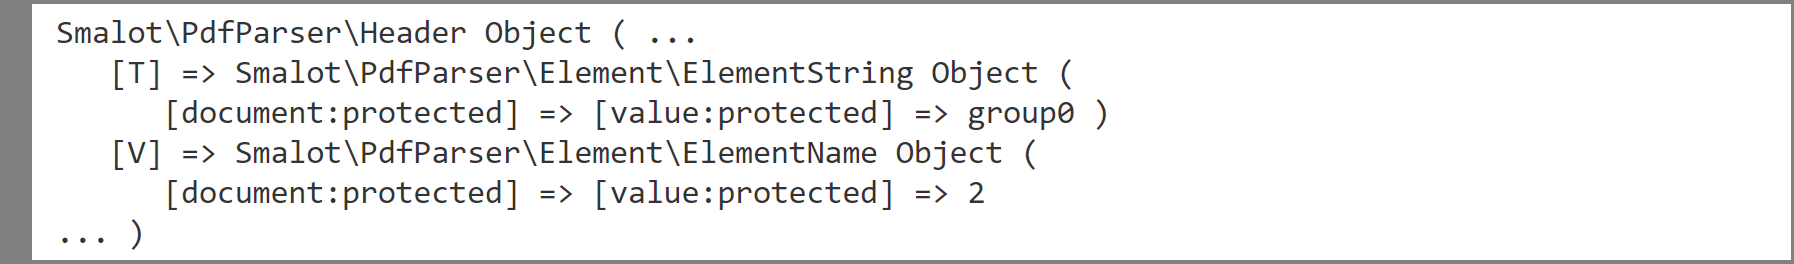
\includegraphics[width=15cm]{img/parsing_object}
\caption{Část dat PDF objektu}
\label{fig:parsing_object}
\end{figure}
\par
K~extrahování dat a zjištění typu formulářového prvku byla vyvinuta metoda \textit{extractElement}, viz výpis \ref{lst:extraction_function}.
\begin{lstlisting}[caption = {Funkční kód pro uložení formulářových prvků z~PDF objektů}, label = {lst:extraction_function}, captionpos=b]
protected function extractElement($header) {
   $elementKey = $header->getElements()['T'];                                                      
   if ($elementKey != null) {
      if (strpos($elementKey->getContent(), 'group') !== false) $type = 'groups';
      else if (strpos($elementKey->getContent(), 'textarea') !== false) $type = 'textareas';
                       
      if ($type != null) {
         $key = $elementKey->getContent();
         $elementValue = $header->getElements()['V'];
         if ($elementValue != null) {
            $value = $elementValue->getContent();
         }    
      }
   }
}
\end{lstlisting}
Kód na samém začátku kontroluje, zda je aktuálně zpracovávaný objekt pojmenován. To je zjištěno na základě indexu \uv{\textbf{T}} (T - Type) v~poli elementů. Pokud název existuje, zjišťuje se, zda se jedná o~textové pole nebo skupinu výběrových tlačítek. Za předpokladu, že typ objektu je validní, je kontrolována hodnota na základě indexu \uv{\textbf{V}} (V~- Value) v~poli elementů. Jakmile objekt obsahuje hodnotu, jsou do parseru vráceny všechny tři hodnoty (název formulářového prvku, typ formulářového prvku a jeho hodnota), které parser uloží do pole všech extrahovaných prvků.

%SECTION
\section{Výsledný vzhled PDF formuláře}
Výsledný vzhled PDF formuláře lze vidět na přiloženém souboru PDF v~příloze \ref{chap:vysledny_vzhled_formulare}. Před formulářem je instrukční text vysvětlující hodnocení prvních osm hodnotících parametrů. Protože se v~některých případech stávalo, že uživatelé otevřeli tento dokument ve webovém prohlížeči, který umožňuje pouze otvírat soubory, nikoliv ukládat, byl zde přidán pokyn využívat prohlížeč PDF Adobe Acrobat, ale je možné využívat i jiné prohlížeče, které podporují vyplňování formulářů. Na konec formuláře byl přidán informační text popisující, jak má uživatel vyplněný formulář nahrát do webového portálu konference TSD.

%SECTION
\section{Technické požadavky}
Technické požadavky pro bezproblémové fungování TCPDI a PDF Parser jsou:
\begin{itemize} 
	\item \verb|PHP verze| -- TCPDI  momentálně funguje na všech verzích PHP, zatímco u~PDF Parseru je potřeba minimální verze 5.3. Proto je nutné mít na serveru PHP verzi alespoň 5.3.0.
	\item \verb|Podpůrné knihovny| -- Při kompresi stránek souborů PDF pomocí knihovny TCPDI je potřeba mít na serveru povoleno rozšíření \textbf{php-zlib}.
	\item \verb|FPDF_TPL verze| -- Aktuální verze TCPDI je kompatibilní pouze s~verzí 1.2.3 knihovny FPDF\_TPL. 
\end{itemize}
